\section{Pianificazione}
Lo sviluppo del progetto è suddiviso nelle seguenti fasi:
\begin{itemize}
    \item RTB;
    \item PB.
\end{itemize}
\subsection{RTB}
Nel periodo dal 04/11/2024 al 17/01/2025 verranno prodotti i seguenti
documenti:
\begin{itemize}
    \item \textit{Norme di progetto};
    \item \textit{Piano di progetto};
    \item \textit{Analisi dei requisiti};
    \item \textit{Piano di qualifica};
    \item \textit{Glossario}.
\end{itemize}
Inoltre verrà realizzato il Proof of Concept (PoC), per valutare la fattibilità tecnologica del progetto.
\subsubsection{Sprint 1 (dal 11/11/2024 al 22/11/2024)}
In questo periodo verrà definito il way of working, documentato nelle
\textit{Norme di progetto}. Per quanto riguarda la gestione di progetto,
verranno pianificate le attività, stilato un preventivo e analizzati i rischi
che potrebbero incidere sullo svolgimento del progetto. Infine, si inizierà a
redigere il \textit{Glossario}, essenziale per garantire una comunicazione
chiara all'interno del team e con il proponente. \\
\begin{figure}[h!]
    \centering
    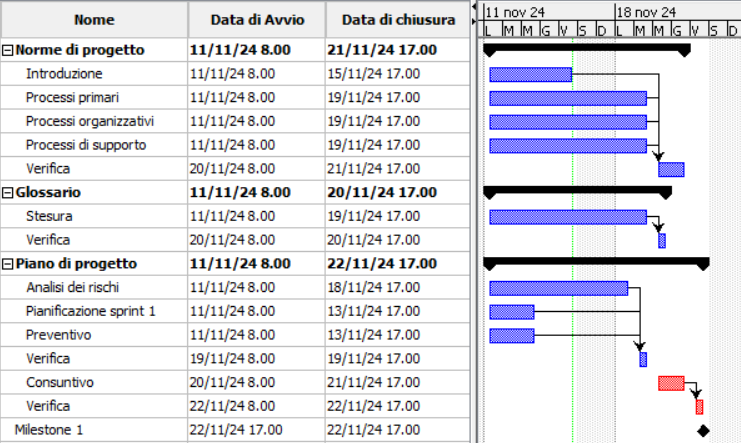
\includegraphics[scale = 0.85]{template/images/gantt1.png}
    \caption{Diagramma di Gantt sprint 1}
    \label{fig:3.1} % Etichetta per il riferimento
\end{figure}
\newpage

\subsubsection{Sprint 2 (dal 25/11/2024 al 06/12/2024)}
Durante questo secondo sprint, ci dedicheremo alla raccolta e all'analisi dei
requisiti, identificando i casi d'uso. Questi saranno documentati nel file
\textit{Analisi dei requisiti} per garantire una visione chiara degli obiettivi
del progetto. Continueremo l'espansione del \textit{Glossario}. Procederemo
inoltre con l'aggiornamento delle \textit{Norme di progetto} per assicurare una
gestione ottimale delle attività e delle risorse. Infine, con priorità minore,
inizieremo la stesura del \textit{Piano di qualifica}, necessario per definire
le metriche e le modalità di verifica della qualità del prodotto.

\begin{figure}[h!]
    \centering
    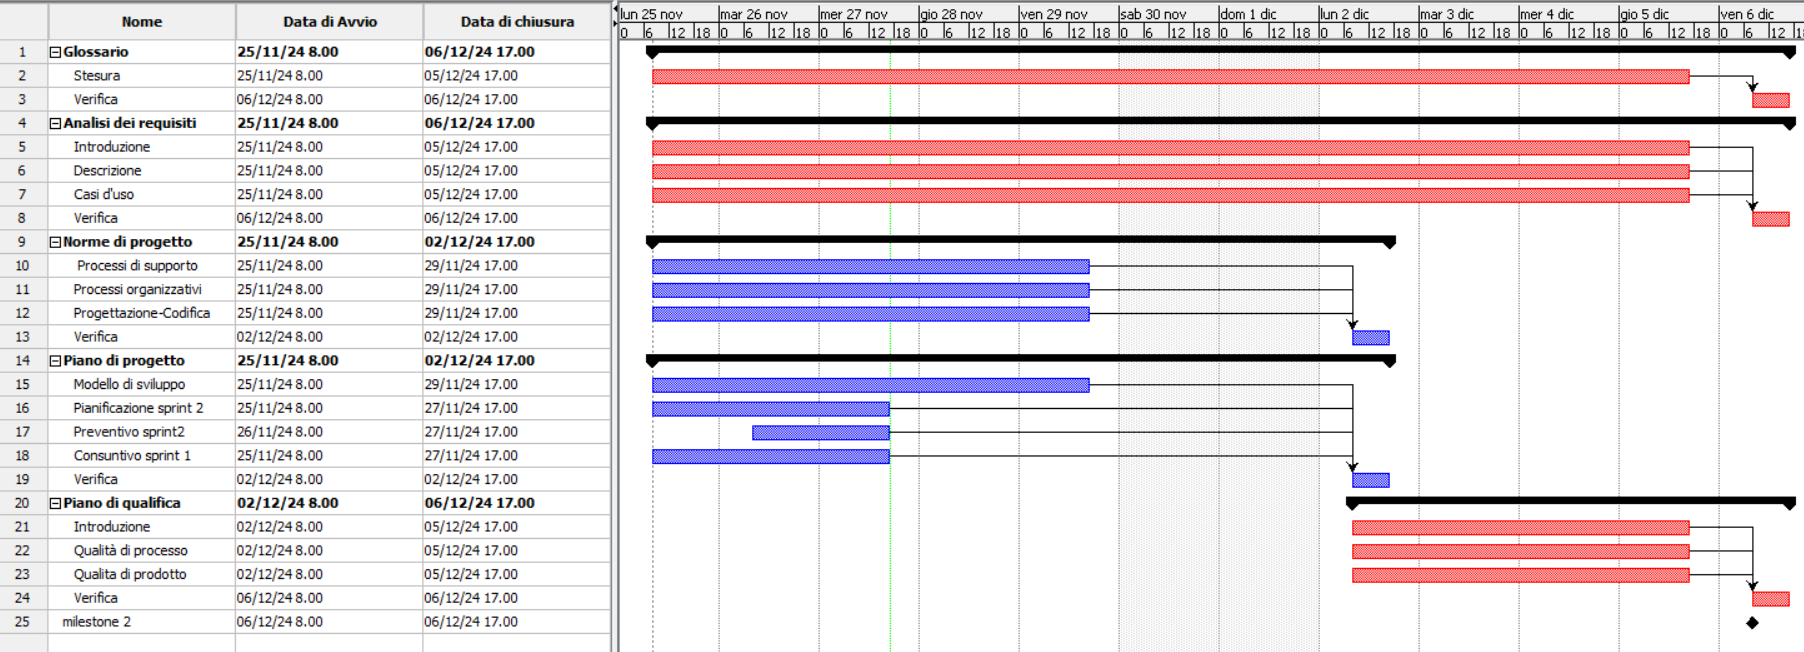
\includegraphics[scale = 0.3]{template/images/gantt2.png}
    \caption{Diagramma di Gantt sprint 2}
    \label{fig:3.2} % Etichetta per il riferimento
\end{figure}

\subsubsection{Sprint 3 (dal 09/12/2024 al 20/12/2024)}
In questo terzo sprint continueremo l'aggiornamento delle \textit{Norme di
    progetto} migliorando le regole che il team si pone di rispettare per garantire
un metodo di sviluppo efficace ed efficiente. E' prevista inoltre la stesura
delle metriche relative alla qualità del progetto e alla qualità del prodotto
nel \textit{Piano di qualifica}. Successivamente, in quanto di minore
importanza, è prevista la stesura della specifica dei test nel medesimo
documento. Per quanto riguarda l'\textit{Analisi dei requisiti} è pianificata
la stesura dei requisiti funzionali e di qualità ed eventualmente, a seguito di
un consulto con il proponente, si procederà anche con la stesura dei requisiti
di vincolo e prestazionali. Infine è prevista l'espansione del
\textit{Glossario}.

\begin{figure}[h!]
    \centering
    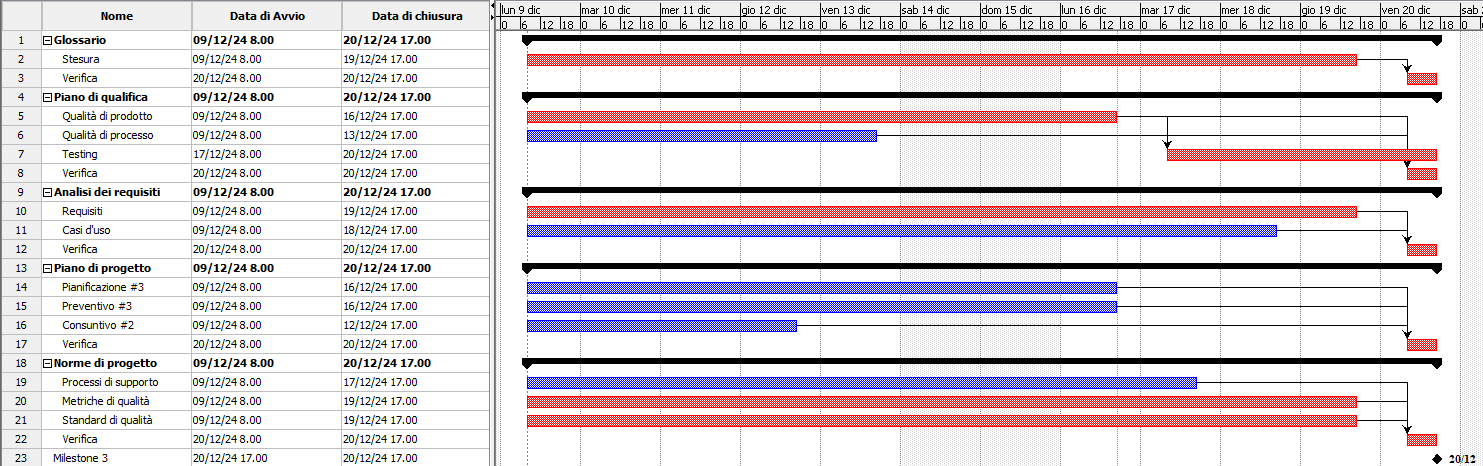
\includegraphics[scale = 0.3]{template/images/gantt3.png}
    \caption{Diagramma di Gantt sprint 3}
    \label{fig:3.3} % Etichetta per il riferimento
\end{figure}
\newpage

\subsubsection{Sprint 4 (dal 23/12/2024 al 10/01/2025)}
Durante questo quarto sprint (di durata maggiore a causa delle festività
natalizie), ci dedicheremo alla sistemazione dei casi d'uso, con l'obiettivo di
garantire che siano coerenti, completi e allineati ai requisiti del progetto.
Una delle attività di maggiore importanza sarà la realizzazione del Proof of
Concept (PoC). Esso servirà a validare le scelte tecniche adottate e a
dimostrare la fattibilità delle soluzioni individuate. Parallelamente, si
cercherà una soluzione per implementare in automatico il controllo della
qualità della documentazione prodotta tramite Indice Gulpease. Infine,
proseguiremo con l'espansione del \textit{Glossario}.

\begin{figure}[h!]
    \centering
    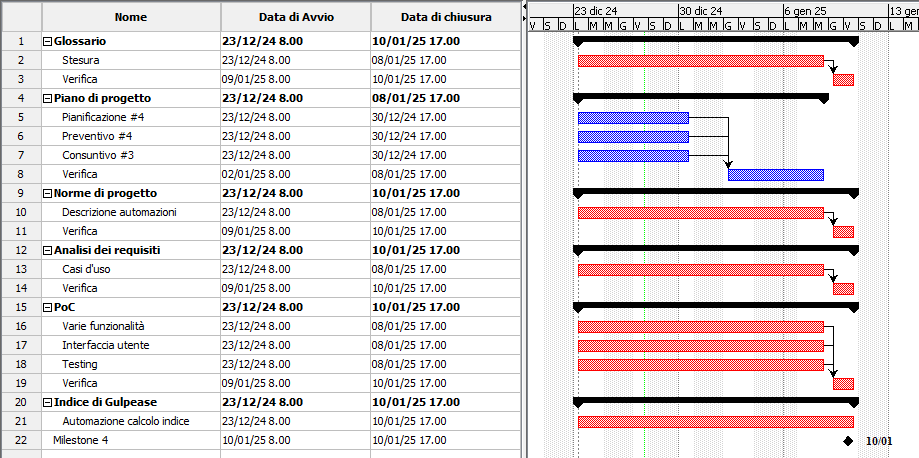
\includegraphics[scale = 0.45]{template/images/gantt4.png}
    \caption{Diagramma di Gantt sprint 4}
    \label{fig:3.4} % Etichetta per il riferimento
\end{figure}

\subsubsection{Sprint 5 (dal 13/01/2025 al 24/01/2025)}
In questo quinto sprint completeremo i documenti necessari per la RTB. Ci
concentreremo sul miglioramento dei documenti con un Indice Gulpease basso.
Vogliamo assicurarci che tutti superino la soglia minima richiesta. Inoltre,
aggiungeremo le sezioni mancanti nelle \textit{Norme di progetto}. Questo
renderà il documento più completo e facile da seguire. Rivedremo anche
l'\textit{Analisi dei requisiti} per migliorarne la chiarezza. Aggiorneremo i
casi d'uso e correggeremo i diagrammi UML per allinearli agli obiettivi del
progetto. Il \textit{Glossario} sarà ampliato con nuovi termini. Questo aiuterà
a rendere il progetto più accessibile. Infine, lavoreremo sul Proof of Concept
(PoC). Risolveremo gli ultimi bug grafici. L'obiettivo è presentare una
versione stabile, chiara e completamente funzionante.

\begin{figure}[h!]
    \centering
    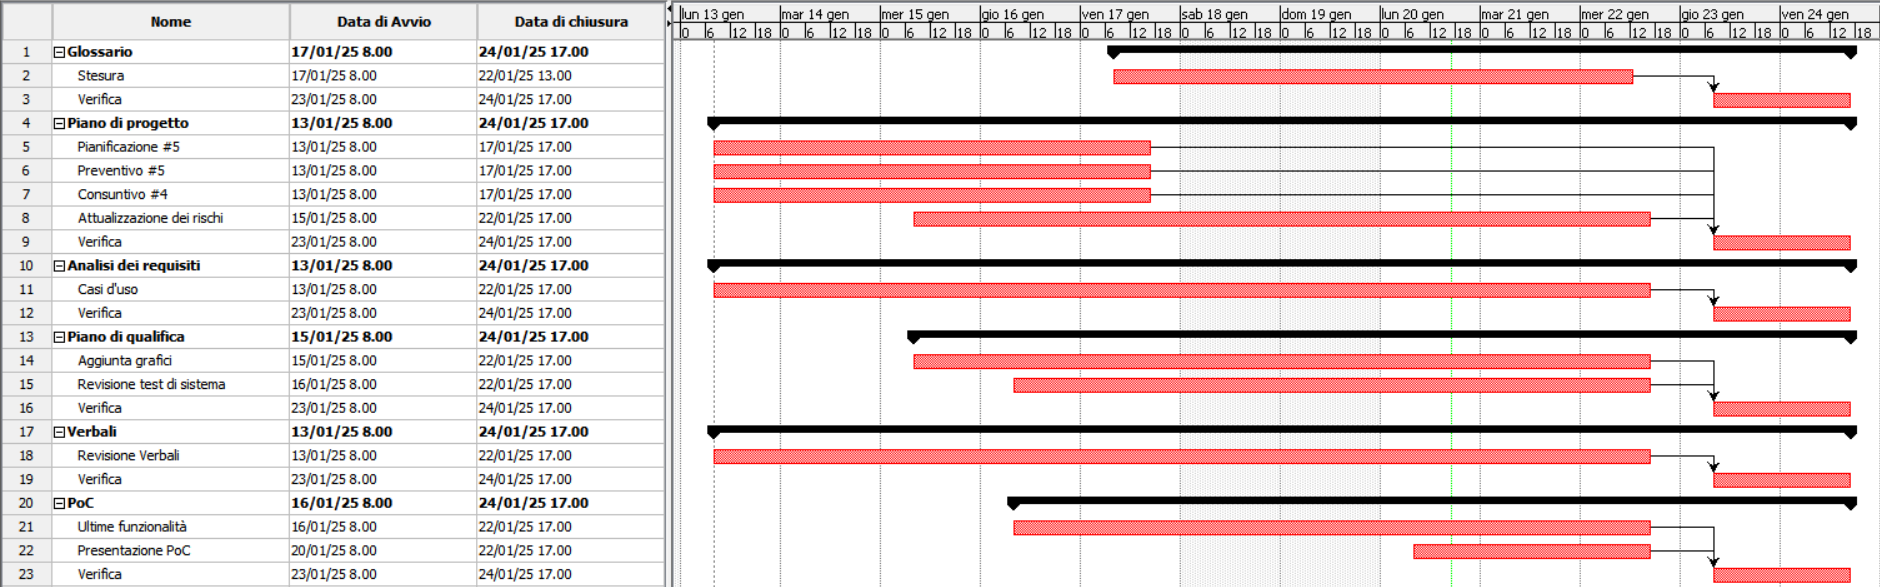
\includegraphics[scale = 0.4]{template/images/gantt5.png}
    \caption{Diagramma di Gantt sprint 5}
    \label{fig:3.5} % Etichetta per il riferimento
\end{figure}
\newpage

\subsubsection{Sprint 6 (dal 27/01/2025 al 07/02/2025)}
In questo sprint, il team si concentrerà sull'approvazione della documentazione
relativa alla RTB. Come passo preliminare, verranno aggiunti i termini mancanti
al documento \textit{Glossario} e verranno eseguite piccole modifiche al
documento \textit{Analisi dei requisiti}. Successivamente, sarà organizzato un
incontro con il professor Cardin Riccardo per presentare il PoC e completare la
prima fase di revisione della RTB. La durata dello sprint sarà quella standard,
sebbene il numero di attività sia inferiore a causa degli impegni di studio dei
membri del team.

\begin{figure}[h!]
    \centering
    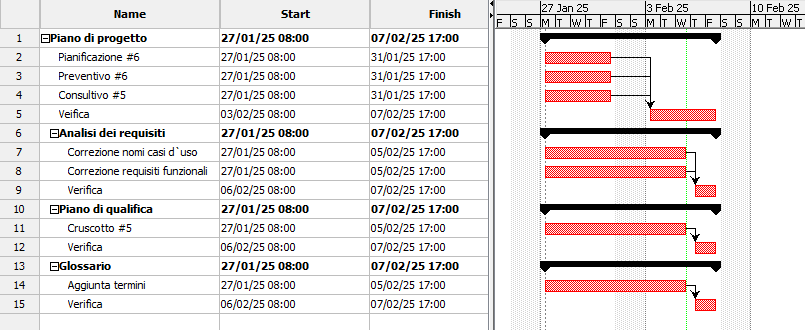
\includegraphics[scale = 0.6]{template/images/gantt6.png}
    \caption{Diagramma di Gantt sprint 6}
    \label{fig:3.6} % Etichetta per il riferimento
\end{figure}

\subsubsection{Sprint 7 (dal 10/02/2025 al 21/02/2025)}
Il settimo sprint sarà dedicato all'integrazione delle tecnologie necessarie
per lo sviluppo del progetto. In particolare, verrà aggiunto il backend al PoC,
che sarà quindi completato; conseguentemente, verrà integrata la lista dei
requisiti di vincolo. Quindi chiederemo un secondo incontro con il professor
Cardin Riccardo per presentare quanto fatto e ricevere un feedback.\\ Inoltre,
verrà redatto il resoconto delle attività di verifica nel \textit{Piano di
qualifica}, relativamente agli sprint 5 e 6. Oltre al \textit{Verbale interno} 
di fine sprint, verrà redatto anche il \textit{Verbale esterno} dell'incontro
del 22-01-2025. Infine, verrà aggiornato il \textit{Glossario} con i nuovi termini introdotti.
\begin{figure}[h!]
    \centering
    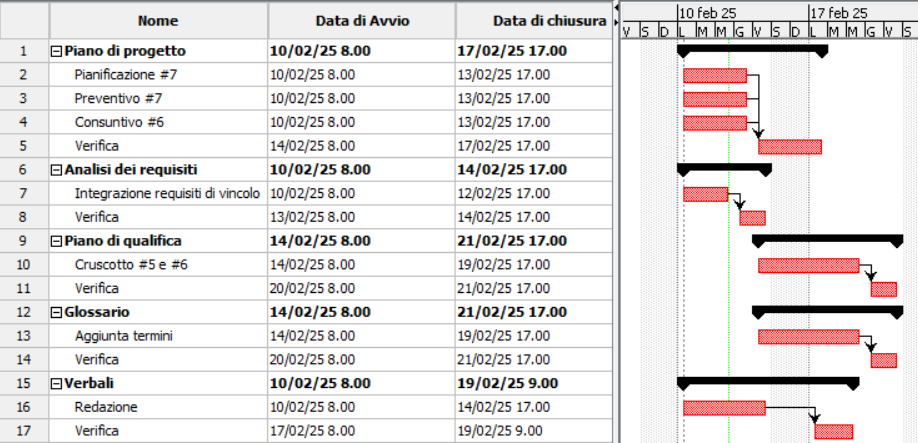
\includegraphics[scale = 0.65]{template/images/gantt7.png}
    \caption{Diagramma di Gantt sprint 7}
    \label{fig:3.7} % Etichetta per il riferimento
\end{figure}
\newpage

\subsubsection{Sprint 8 (dal 24/02/2025 al 27/02/2025)}
Durante l'ottavo sprint, ci dedicheremo al perfezionamento dell'organizzazione del repository e all'ottimizzazione della GitHub Page.
Affronteremo anche le eventuali modifiche all'\textit{Analisi dei requisiti} suggerite dal professor Riccardo Cardin.
Inoltre, è in programma un incontro con il proponente per un approfondimento sulle prestazioni del software e sulle soluzioni tecniche adottate.
Data la ridotta mole di lavoro restante per la presentazione dell'RTB, questo sprint avrà una durata di una sola settimana.

\begin{figure}[h!]
    \centering
    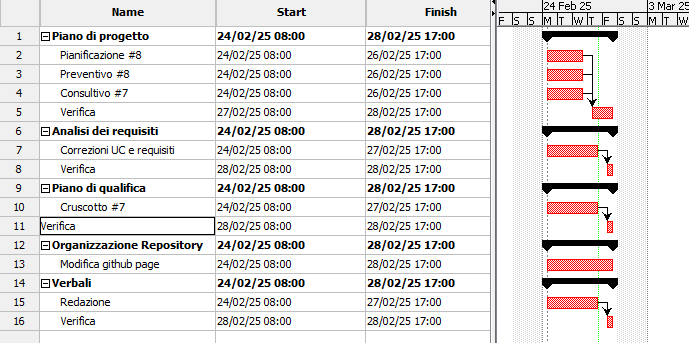
\includegraphics[scale = 0.7]{template/images/gantt8.png}
    \caption{Diagramma di Gantt sprint 8}
    \label{fig:3.8} % Etichetta per il riferimento
\end{figure}

\subsection{PB}
A seguito dell'esito dell'RTB il gruppo procederà con la seconda fase del progetto, ossia la PB (Product Baseline).
Nel periodo dal 17/03/2025 verranno creati i seguenti documenti:
\begin{itemize}
    \item \textit{Specifica tecnica}
    \item \textit{Manuale utente}
\end{itemize}
Verranno inoltre corretti e aggiornati i documenti della fase precedente.
Verrà realizzato il Minimun Viable Product (MVP), ossia un prodotto software in grado di soddisfare tutte le funzionalità richieste dal proponente.

\subsubsection{Sprint 9 (dal 17/03/2025 al 28/03/2025)}
In questo periodo, il team si concentrerà sullo studio della progettazione software, approfondendo i pattern per l’implementazione di back-end e front-end.
Verranno inoltre apportate delle modifiche ai documenti segnalati dall'esito RTB.
Il team si impegnerà ad icrementare notevolmente le ore produttive in modo da rispettare i tempi programmati per la fine del progetto didattico.


\begin{figure}[H]
    \centering
    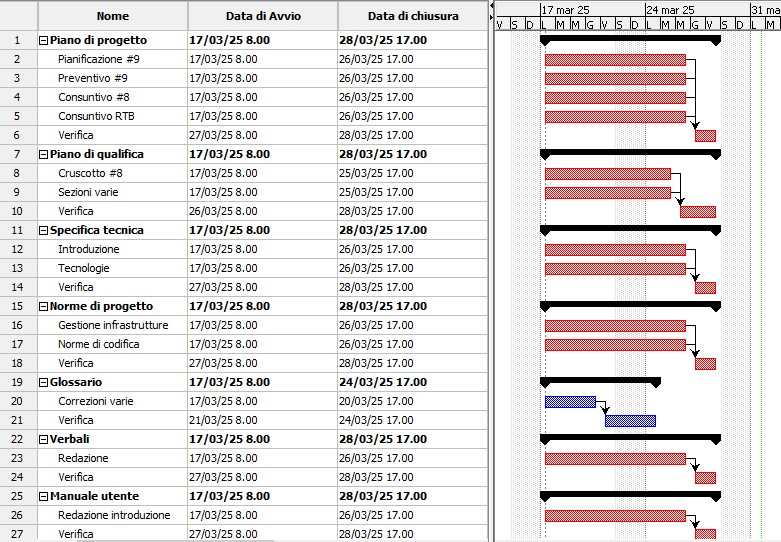
\includegraphics[scale = 0.5]{template/images/gantt9.png}
    \caption{Diagramma di Gantt sprint 9}
    \label{fig:3.9} % Etichetta per il riferimento
\end{figure}

\subsubsection{Sprint 10 (dal 31/03/2025 al 11/04/2025)}  
L'obiettivo principale di questo sprint è completare la progettazione di dettaglio del backend e del frontend. In particolare concluderemo la creazione dei diagrammi UML e la redazione della sezione relativa all'architettura nella
 \textit{Specifica tecnica}. Dopodiché inizieremo la codifica del software a partire dalla configurazione dell'ambiente di sviluppo e dall'implementazione delle action per la CI.
In parallelo, aggiorneremo i documenti \textit{Norme di progetto}, \textit{Piano di qualifica} e \textit{Analisi dei requisiti}.
\begin{figure}[h!]
    \centering
    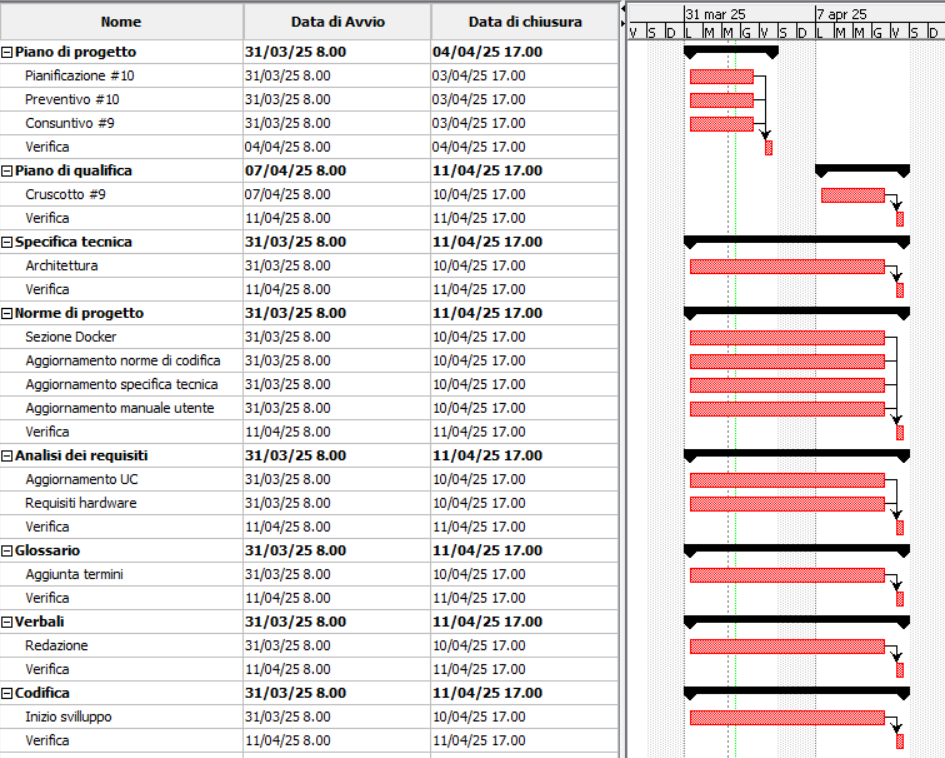
\includegraphics[scale = 0.45]{template/images/gantt10.png}
    \caption{Diagramma di Gantt sprint 10}
    \label{fig:3.10} % Etichetta per il riferimento
\end{figure}

\subsubsection{Sprint 11 (dal 14/04/2025 al 25/04/2025)}
L’obiettivo principale di questo sprint è completare la codifica dell'MVP e finalizzare la documentazione in vista della PB. I membri del team concentreranno la maggior parte delle risorse temporali sul raggiungimento di questo traguardo.
In parallelo, verrà ultimata la stesura della \textit{Specifica tecnica}, e avvieremo la redazione del \textit{Manuale utente}, con l’intenzione di completarlo entro la fine dello sprint.
Saranno inoltre aggiornati i documenti \textit{Norme di progetto} e \textit{Piano di qualifica}.
\begin{figure}[h!]
   \centering
    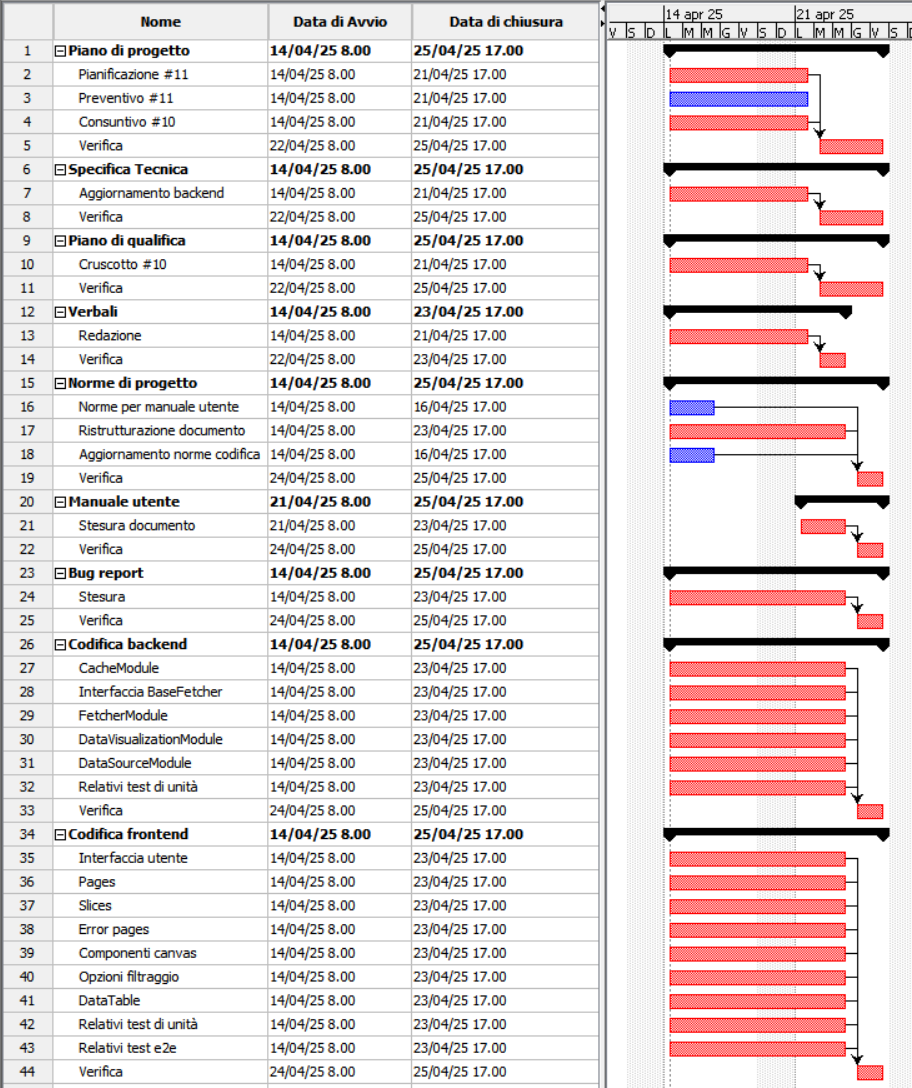
\includegraphics[scale = 0.5]{template/images/gantt11.png}
    \caption{Diagramma di Gantt sprint 11}
    \label{fig:3.10} % Etichetta per il riferimento
\end{figure}
\subsubsection{Sprint 12 (dal 28/04/2025 al 02/05/2025)}
L'obiettivo dello sprint è concludere il progetto affrontando la revisione PB. A tal fine, le attività principali saranno il completamento della stesura dei documenti \textit{Specifica tecnica}, \textit{Piano di progetto} e \textit{Piano di qualifica}, oltre all'approvazione dei documenti rimanenti.
\begin{figure}[h!]
   \centering
    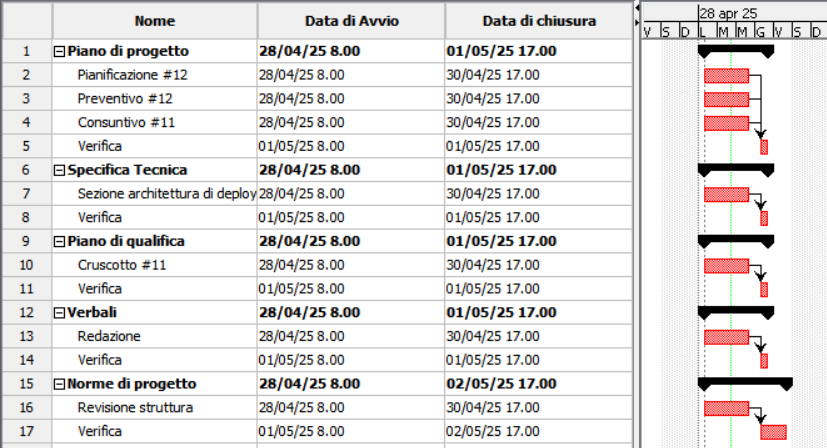
\includegraphics[scale = 0.5]{template/images/gantt12.png}
    \caption{Diagramma di Gantt sprint 12}
    \label{fig:3.10} % Etichetta per il riferimento
\end{figure}